\documentclass[12pt]{article}
\usepackage{ctex}
% \usepackage[margin=1.25in]{geometry}
\usepackage[inner=2.0cm,outer=2.0cm,top=2.5cm,bottom=2.5cm]{geometry}
\usepackage{color}
\usepackage{graphicx}
\usepackage{amssymb}
\usepackage{amsmath}
\usepackage{amsthm}
\usepackage{bm}
\usepackage{hyperref}
\usepackage{multirow}
\usepackage{mathtools}
\usepackage{enumerate}


\newcommand{\homework}[5]{
	\pagestyle{myheadings}
	\thispagestyle{plain}
	\newpage
	\setcounter{page}{1}
	\noindent
	\begin{center}
		\framebox{
			\vbox{\vspace{2mm}
				\hbox to 6.28in { {\bf KRP \hfill #2} }
				\vspace{6mm}
				\hbox to 6.28in { {\Large \hfill #1 \hfill} }
				\vspace{6mm}
				\hbox to 6.28in { {\it Instructor: {\rm #3} \hfill Name: {\rm #4}, StudentId: {\rm #5}}}
				\vspace{2mm}}
		}
	\end{center}
	% \markboth{#4 -- #1}{#4 -- #1}
	\vspace*{4mm}
}


\begin{document}
\large
	%==========================Put your name and id here==========================
	\homework{Homework 3}{Spring 2023}{YiZheng Zhao}{张运吉}{211300063}
    \paragraph{Question 1. Closure under Disjoint Union}~{}
    \\

    Let $C$ be an $\mathcal{ALC}$-Concept. If there exists a rule that can be applied, then $C$ has a subconcept of the form $\lnot D$, and $D$ is as the form of $E \sqcap F, E \sqcup F, \lnot E, \exists r.E,\forall r.E$. Let $C'$ be the $\mathcal{ALC}$-concept after rule application.
    \begin{itemize}
        \item case 1: $\lnot D = \lnot (E \sqcap F)$, $E, F$ is concept name.  \\
        After transforming, $\lnot (E \sqcap F)$ became $\lnot \lnot \lnot E \sqcup \lnot \lnot \lnot F$.
    \begin{equation}
        \begin{aligned}
            M(\lnot (E \sqcap F)) &= \{ \#(E \sqcap F) \} \cup M(E) \cup M(F) \\
            M(\lnot \lnot \lnot E \sqcup \lnot \lnot \lnot F) &= \{ \#(\lnot \lnot E), \#(\lnot E), \#E, \#(\lnot \lnot F), \#(\lnot F), \#F \} \\
            & \quad \cup M(E) \cup M(F) \\
            M(C') &= (M(C) \setminus M(\lnot D)) \cup M(\lnot \lnot \lnot E \sqcup \lnot \lnot \lnot F) \\ &= (M(C) \setminus \{ \#(E \sqcap F) \}) \\ &\quad \cup \{ \#(\lnot \lnot E), \#(\lnot E), \#E, \#(\lnot \lnot F), \#(\lnot F), \#F \}
            \nonumber
        \end{aligned}
    \end{equation} 
    So, we can get that after transforming, $\#(E \sqcap F)$ was replaced by some smaller numbers $\#(\lnot \lnot E), \#(\lnot E), \#E, \#(\lnot \lnot F), \#(\lnot F), \#F$.
    \item case 2: $\lnot D = \lnot (E \sqcup F)$, $E, F$ is concept name. \\
    The prove of case 2 is similar as case 1.
    \item case 3: $\lnot D = \lnot \lnot E$, $E$ is a concept name. \\
    After transforming, $\lnot \lnot E$ became $E$. \\
    \begin{equation}
        \begin{aligned}
            M(\lnot  \lnot E) &= \{ \# \lnot E, \# E\} \\ 
            M(C') &= (M(C) \setminus M(\lnot \lnot E)) \cup M(E) = M(C) \setminus \{ \# \lnot E, \#E \} \\
            \nonumber
        \end{aligned}
        \nonumber
    \end{equation}
    So, we can get that after transforming, $\# \lnot E, \# E$ was deleted.
    \item case 4: $\lnot D = \lnot (\exists r.E)$, $E$ is a concept name. \\
    \begin{equation}
        \begin{aligned}
            M(\lnot (\exists r.E)) &= \{ \#(\exists r.E) \} \cup M(E) \\
            M(\forall r.\lnot E) &= \{ \#E \} \cup M(E) \\
            M(C') &= (M(C) \setminus M(\lnot (\exists r.E))) \cup M(\forall r.\lnot E) = (M(C) \setminus \{ \#(\exists r.E) \}) \cup \{ \#E \}
            \nonumber
        \end{aligned}
    \end{equation}
    So, we can get that after transforming, $\#(\exists r.E)$ was replaced by a smaller number $\#E$.
    \item case 5: $\lnot D = \lnot (\forall r.E)$, $E$ is a concept name. \\
    The prove of case 5 is similar as case 4.
    \end{itemize}
    Finally, we can get that with transforming, the elements of $M(C)$ will became smaller over and over again, the stop condition is the elements of $M(C)$ all becomes $0$.  The procedure of transformations is always terminates because the numbers are limited.\\

    \paragraph{Question 2. Negation Normal Norm (NNF)}~{}
    \\
    \begin{enumerate}
    \item[(1)]
	$\Longrightarrow$: \par
    let $\mathcal{T}^{'}$ is obtained from $\mathcal{T}$ by replacing each concept defnition $A \equiv C$ with the concept inclusion $A \sqsubseteq C$ and $C \sqsubseteq A$, $\mathcal{T}$ is equivalent to $\mathcal{T}'$. \par
    Obviously, $\mathcal{T}^{\sqsubseteq} \subseteq \mathcal{T}'$, which means any model of $\subseteq \mathcal{T}'$ is also a model of $\mathcal{T}^{\sqsubseteq}$.\par
    So, every concept name is satisfable w.r.t. $\mathcal{T}$ implies it is satisfable w.r.t. $\mathcal{T}^{\sqsubseteq}$.\par
    $\Longleftarrow$: \par
    If concept name $C$ is satisfiable w.r.t. $\mathcal{T}^{\sqsubseteq}$ , then there exists an interpretation $\mathcal{I}$  s.t. $C^{\mathcal{I}}\not = \emptyset$ w.r.t. $\mathcal{T}^{\sqsubseteq}$. \par
    We expand $\mathcal{I}$ and get $\mathcal{J}$. 
    The rule to expand is as follow: We modify recursively all $A^{\mathcal{J}^{}},C_1^{\mathcal{J}},C_2^{\mathcal{I}}……,C_n^{\mathcal{J}}$ to $A^{\mathcal{I}}\cup \ C_1^{\mathcal{I}}\cup \ C_2^{\mathcal{I}}\cup……\cup \ C_n^{\mathcal{I}} \text { if GCI }  A \sqsubseteq C_i \text { in } \mathcal{T} ^\sqsubseteq $ for all $1\le i\le n,$ until all $A^{\mathcal{J}^{}} =\ C^{\mathcal{J}} \text { if concept defnition } A \equiv C \text { in } \mathcal{T}$. \par
    Because the stop condition is $A^{\mathcal{J}^{}} =\ C^{\mathcal{J}}$ and the expand procedure does not violate any one GCI, so $\mathcal{J}$ is a interpretation w.r.t. $\mathcal{T}$. Because we just expand some $A^{\mathcal{I}}$ and get corresponding $A^{\mathcal{J}}$, so $C^{\mathcal{J}} \neq \emptyset$ due to $C^{\mathcal{I}} \neq \emptyset$.\par
    Therefore, $C$ is satisfiable w.r.t. $\mathcal{T}$.
    \item[(2)]
    Do not holds. \par
    \begin{equation}
        \begin{aligned}
            \mathcal{T} &= \{ A \equiv C \sqcap \lnot B, B \equiv P, C \equiv P \} \\
            \mathcal{T}^{\sqsubseteq} &= \{ A \sqsubseteq C \sqcap \lnot B, B \sqsubseteq P, C \sqsubseteq P \} \nonumber
        \end{aligned}
    \end{equation}
    Because: 
    \begin{equation}
        A^{\mathcal{I}} = (C \sqcap \lnot B)^{\mathcal{I}} = C^{\mathcal{I}} \cap (\Delta^{\mathcal{I}} \setminus B^{\mathcal{I}}) = P^{\mathcal{I}} \cap (\Delta^{\mathcal{I}} \setminus P^{\mathcal{I}}) = \emptyset \nonumber
    \end{equation}
    So concept name $\mathcal{A}$ is not satisfiable w.r.t. $\mathcal{T}$.\par
    Let $\Delta^{\mathcal{I}} = \{ a \}, A^{\mathcal{I}} = \{ a \}, C^{\mathcal{I}} = \{ a \}, B^{\mathcal{I}} = \empty, P^{\mathcal{I}} = \{ a \}$, obviously it satisfies $T^{\sqsubseteq}$ and $A^{\mathcal{I}}\neq \emptyset$.\par
    So concept name $A$ is satisfiable w.r.t. $\mathcal{T}^{\sqsubseteq}$.
    \end{enumerate}

    \paragraph{Question 3. Tableau Algorithm for ABoxes with Acyclic TBoxes}~{}
    \\

    \begin{itemize}
        \item Termination. \par
        We had known that the tableau algorithm consistent($\mathcal{A}$) is terminate, so we only need to prove that after using $\equiv_{1}$-rule and $\equiv_{2}$-rule to unfold $\mathcal{T}$, the new Abox $\mathcal{A}^{'}$ is finite. Obviously, we would add finite number of assertions to $\mathcal{A}$, so the new Abox $\mathcal{A}^{'}$ is finite.
        \item Soundness. \par
        Let $\mathcal{A}^{'}$ = consistent($\mathcal{K}$, $\mathcal{A}$).To construct a model from a complete and clash-free ABox $\mathcal{A}^{'}$, we can use the same definitions as presented in the lecture slides to obtain an interpretation $\mathcal{J}$ of all role names and of the concept names that do not have definitions in $\mathcal{T}$. It remains to show that $\mathcal{J}$ is also a model of $\mathcal{A}^{'}$, where the main problem is showing Property (P1) by induction. So let's prove it.\par
        If $C$ doesn't have definition in $\mathcal{T}$, then we have already
        proved it. Otherwise $C$ has definition. According to the $\equiv_{1}$-rule and $\equiv_{2}$-rule, if $a : A$ and $A \equiv C$, there must be $a : C$ in $\mathcal{A}^{'}$, if $a : \neg A$ and $A \equiv C$, there must be $a: \dot{\neg} C$, by the defnition of $\mathcal{J}$, $a^{\mathcal{J}} \in A^{\mathcal{J}}$.
        \item Completeness. \par
        The $\equiv_{1}$-rule: if $a : A \in A$, $A \equiv C \in \mathcal{T}$, then $a^\mathcal{I} \in A^{\mathcal{I}}$, $A^\mathcal{I} = C^{\mathcal{I}}$, so $a^\mathcal{I} \in C^{\mathcal{I}}$. Therefore, $\mathcal{I}$ is still a model of $\mathcal{A} \cup \{a : C\}$.\par
        The $\equiv_{2}$-rule: if $a : \neg A \in A$, $A \equiv C \in \mathcal{T}$, then $a^\mathcal{I} \not \in A^{\mathcal{I}}$, $A^\mathcal{I} = C^{\mathcal{I}}$, so $a^\mathcal{I} \not \in C^{\mathcal{I}}$. Therefore, $\mathcal{I}$ is still a model of $\mathcal{A} \cup \{a : \dot \neg C\}$. \par
        The other rules are as the same as presented in the text book.
    \end{itemize}
    Therefore, consistent$(\mathcal{T} , \mathcal{A})$ is a decision procedure for the consistency of $\mathcal{ALC}$-knowledge bases with acyclic TBoxes.
    \paragraph{Question 4. Tableau Algorithm for ABoxes with Acyclic TBoxes}~{}
    \\

    Doesn't hold. \par
    If the subsumption $\neg(\forall r . A) \sqcap \forall r . C \sqsubseteq \forall r . E$ doesn't hold w.r.t. acyclic TBox $\mathcal{T}$, then $\neg(\forall r . A) \sqcap \forall r . C \sqcap \neg(\forall r . E)$ holds w.r.t. acyclic TBox $\mathcal{T}$. \par
    We use tableau algorithm to determine it.\par
    \begin{equation}
        \begin{aligned}
            \mathcal{A}_{0} &=\{a: \neg(\forall r . A) \sqcap \forall r . C \sqcap \neg(\forall r . E)\} \\
            \mathcal{A}_{1} &=\mathcal{A}_{0} \cup\{a: \neg(\forall r . A), a: \forall r . C, a: \neg(\forall r . E) \\ & =\mathcal{A}_{0} \cup\{a: \exists r . \neg A, a: \forall r . C, a: \exists r . \neg E\} \quad (\sqcap \text{-rule}) \\
            \mathcal{A}_{2}&=\mathcal{A}_{1} \cup\{(a, b): r, b: \neg A,(a, c): r, c: \neg E\} \quad(\exists \text{-rule})\\
            \mathcal{A}_{3} &=\mathcal{A}_{2} \cup\{b: C, c: C\} \quad(\forall\text{-rule})\\
            \mathcal{A}_{4}&=\mathcal{A}_{3} \cup\{b:(\exists r . \neg B) \sqcap \neg A, c:(\exists r . \neg B) \sqcap \neg A\} \quad(\equiv_{1}\text{-rule})\\
            \mathcal{A}_{5}&=\mathcal{A}_{4} \cup\{c: \exists r . A \sqcup \forall r . \neg D\} \quad(\equiv_{2}\text{-rule})\\
            \mathcal{A}_{6}&=\mathcal{A}_{5} \cup\{b: \exists r . \neg B, c: \exists r . \neg B, c: \neg A\} \quad (\sqcap \text{-rule})\\
            \mathcal{A}_{7}&=\mathcal{A}_{6} \cup\{(b, d): r, d: \neg B,(c, e): r, e: \neg B\} \quad(\exists \text{-rule})\\
            \mathcal{A}_{8}&=\mathcal{A}_{7} \cup\{c: \exists r . A\} \quad (\sqcup\text{-rule})  \\
            \mathcal{A}_{9}&=\mathcal{A}_{8} \cup\{(c, f): r, f: A\} \quad(\exists \text{-rule})\\
            \nonumber
        \end{aligned}
    \end{equation}
    There is no rules to apply in $\mathcal{A}_9$ and it is clash free, which means $\neg(\forall r . A) \sqcap \forall r . C \sqcap \neg(\forall r . E)$ holds w.r.t. acyclic TBox $\mathcal{T}$ and $\neg(\forall r . A) \sqcap \forall r . C \sqsubseteq \forall r . E$ doesn't hold w.r.t. acyclic TBox $\mathcal{T}$

    \paragraph{Question 5. Anywhere Blocking}~{}
    \\
    \begin{itemize}
        \item Termination. \par
        Let $m = |\operatorname{sub}(K)|$. Termination is a consequence of the following properties of the expansion rules: \par
        (1) There can be at most $|\operatorname{sub}(\mathcal{K})|$ rule applications of a individual name. \par
        (2) The outdegree of each tree in the forest-shaped $\mathrm{ABox}$ is bounded by $|\operatorname{sub}(\mathcal{K})|$. \par
        (3) Any path having more individual names than $2^{|\operatorname{sub}(\mathcal{K})|}$ has at least two individual names $a, b$ such that $\operatorname{con}_{\mathcal{A}}(b)=\operatorname{con}_{\mathcal{A}}(a) \subseteq \operatorname{sub}(\mathcal{K})$. Because the ages of a individual name are strictly monotonic increasing, we assume that age $(a)<$ age(b). Therefore, there are at most $2^m$ individual names in a path along tree individuals that are not blocked. That means the depth of each tree in the forest-shaped $ABox$ is bounded by $2^m$.
        \item Soundness. \par
        Let $\mathcal{A}^{'}$ = consistent($\mathcal{K})$. We firstly construct $\mathcal{A}^{'}$:
        \begin{equation}
            \begin{aligned} \mathcal{A}^{\prime \prime}= & \left\{a: C \mid a: C \in \mathcal{A}^{\prime} \text { and } a \text { is not blocked }\right\} \cup \\ & \left\{(a, b): r \mid(a, b): r \in \mathcal{A}^{\prime} \text { and } b \text { is not blocked }\right\} \cup \\ & \left\{\left(a, b^{\prime}\right): r \mid(a, b): r \in \mathcal{A}^{\prime}, a \text { is not blocked and } b \text { is blocked by } b^{\prime}\right\}\end{aligned}
            \nonumber
        \end{equation}
        The first preconclusion we want to show is: 
        \begin{equation}
            \operatorname{con}_{\mathcal{A}^{\prime\prime}}(a)=\operatorname{con}_{\mathcal{A}^{\prime}}(a)
            \nonumber
        \end{equation} \par
        \begin{itemize}
            \item For individual assertion, $a$ must not be blocked by its definition.
            \item For role assertion, there is two case: \\
            case 1: $(a, b) \in r \in \mathcal{A}^{'}$, because the successor of a blocked individual is also blocked, so $a$ must not be blocked. \\
            case 2: $(a, b^{'}) \not\in r \in \mathcal{A}^{'}$, $b^{\prime}$ is not blocked according to the definition of anywhere blocking.
        \end{itemize} \par
        Therefore, there is no blocked individual names in $\mathcal{A}^{\prime\prime}$, which means the fir  preconclusion holds. \par
        The second preconclusion we want to show is:
        \begin{equation}
            \mathcal{A}^{\prime\prime} \text{ is complete if } \mathcal{A}^{\prime} \text{ is complete. }
            \nonumber
        \end{equation}
        \begin{itemize}
            \item $\sqcap-$ rule: if $a: C \sqcap D \in \mathcal{A}^{\prime \prime}$, according to the first preconclusion $a: C \sqcap D \in \mathcal{A}^{\prime}$. Completeness of $\mathcal{A}^{\prime}$ implies that $\{a: C, a: D\} \subseteq \mathcal{A}^{\prime}$ and then the first preconclusion implies $\{a: C, a: D\} \subseteq \mathcal{A}^{\prime \prime}$.
            \item $\sqcup-$ rule: if $a: C \sqcup D \in \mathcal{A}^{\prime \prime}$, according to the first preconclusion $a: C \sqcup D \in \mathcal{A}^{\prime}$. Completeness of $\mathcal{A}^{\prime}$ implies that at least one of $\{a: C, a: D\}$ is in $\mathcal{A}^{\prime}$ and then the first preconclusion implies at least one of $\{a: C, a: D\}$ is in $\mathcal{A}^{\prime \prime}$.
            \item $\sqsubseteq-$ rule: if $C \sqsubseteq D \in \mathcal{T}$ and $a: C \in \mathcal{A}^{\prime \prime}$, according to the first preconclusion $a: C \sqsubseteq D \in \mathcal{A}^{\prime}$. Completeness of $\mathcal{A}^{\prime}$ implies that $a: D \in \mathcal{A}^{\prime}$ and then the first preconclusion implies $a: D \in \mathcal{A}^{\prime \prime}$.
            \item $\exists-$ rule: if $a: \exists r . C \in \mathcal{A}^{\prime \prime}$, according to the first preconclusion $a: \exists r . C \in \mathcal{A}^{\prime}$ and $a$ is not blocked in $\mathcal{A}^{\prime}$. Completeness of $\mathcal{A}^{\prime}$ implies that $\{(a, b): r, b: C\} \subseteq \mathcal{A}^{\prime}$. If $b$ is not blocked, $\{(a, b): r, b: C\} \subseteq \mathcal{A}^{\prime\prime}$ according to the definition of $\mathcal{A}^{\prime \prime}$. If $b$ is anywhere blocked by $b^{\prime}$, then $b^{\prime}$ is not blocked and $\operatorname{con}_{\mathcal{A}^{\prime}}(b) \subseteq$ con $_{A^{\prime}}\left(b^{\prime}\right)$ according to the definition of anywhere blocking. Therefore, $b^{\prime}: C \in \mathcal{A}^{\prime \prime}$ according to the first preconclusion. By definition of $\mathcal{A}^{\prime \prime}$, we have $\left(a, b^{\prime}\right): r \in \mathcal{A}^{\prime \prime}$ naturally. 
            \item $\forall$-rule: if $\left\{a: \forall r . C,\left(a, b^{\prime}\right): r\right\} \subseteq \mathcal{A}^{\prime \prime}$, then $a: \forall r . C \in \mathcal{A}^{\prime}$ and neither $a$ or $b^{\prime}$ not blocked in $\mathcal{A}^{\prime}$. If $\left(a, b^{\prime}\right): r \in \mathcal{A}^{\prime}$, then completeness of $\mathcal{A}^{\prime}$ implies $b^{\prime}: C \in \mathcal{A}^{\prime \prime}$. If $\left(a, b^{\prime}\right): r \notin \mathcal{A}^{\prime}$, then there must be a $b$ such that $(a, b): r \in \mathcal{A}^{\prime}$ and $b$ is anywhere blocked by $b^{\prime}$ in $\mathcal{A}^{\prime}$. Then completeness of $\mathcal{A}^{\prime}$ implies $b: C \in \mathcal{A}^{\prime}$. According to the definition of anywhere blocking, we have $\operatorname{con}_{A^{\prime}}(b) \subseteq \operatorname{con}_{A^{\prime}}\left(b^{\prime}\right)$, and $b^{\prime}: C \in \mathcal{A}^{\prime}$. Then the first preconclusion implies that $b^{\prime}: C \in A^{\prime \prime}$.
        \end{itemize}
        Now, we can construct a interpretation $\mathcal{I}$ according to $\mathcal{A}^{\prime \prime}$ just like the prove of lemma 4.5 in the text book and then we can get that $\mathcal{I}$ is a model of $\mathcal{A}^{''}$ and $\mathcal{A}$. \par
        For each GCI $C \sqsubseteq D \in \mathcal{T}$ and assertion $a: C \in \mathcal{A}$, we have $a: C \in \mathcal{A}^{\prime \prime}$ and $a: D \in \mathcal{A}^{\prime \prime}$. If $a^\mathcal{I} \in C^\mathcal{I}$, then $a^\mathcal{I} \in D^\mathcal{I}$ and thus $C^\mathcal{I} \subseteq D^\mathcal{I}$. Therefore, $\mathcal{I}$ is a model of $\mathcal{T}$. \par
        To sum up, $\mathcal{I}$ is a model of $\mathcal{K} = (\mathcal{T}, \mathcal{A})$, $\mathcal{K}$ is consistent if the tableau algorithm with anywhere blocking returns "consistent".
        \item Completeness. \par
        The prove of completeness is similar as the prove on the text book. The only difference is   $\sqsubseteq$-rule: If $a: C \in \mathcal{A}$ and $C \sqsubseteq D \in \mathcal{T}$, then $a^\mathcal{I} \in C^I$ and $C^\mathcal{I} \sqsubseteq D^\mathcal{I}$ by semantics. Consequently, adding $a: D$ to $\mathcal{A}$ has no effect on the consistency of $\mathcal{K}$. Therefore, $\mathcal{I}$ is still a model of $(\mathcal{T}, \mathcal{A} \cup\{a: D\})$.
    \end{itemize}

    \paragraph{Question 6. Precompletion of Tableau Algorithm}~{}
    \\

    $\Longrightarrow:$ \par
    Let $\mathcal{J}$ denote a model of $\mathcal{K}$. According to the completeness of tableau algorithm, applying any rule to $\mathcal{A}$ will not change the consistency of $\mathcal{K}$ for any model with respect to $\mathcal{K}$. Therefore, $\mathcal{J}$ is also a model with respect to $\mathcal{A}^{\prime}$(precompletion of $\mathcal{K}$). \par
    By the definition of $C_{\mathcal{A}}^a$, obviously $a^\mathcal{J} \in C_{\mathcal{A}^{\prime}}^a$. So $C_{\mathcal{A}^{'}}^a$ is satisfiable with respect to $\mathcal{T}$ for each individual name $a$ that occurs in $\mathcal{A}^{\prime}$. \par
    $\Longleftarrow:$ \par
    We construct a suitable interpretation $I$: 

    - $\Delta^I$ = \{a | $a:C \in \mathcal{A}^{\prime}\}$

    - $a^I=a$ for all individual name $a$ in $\mathcal{A}^{\prime}$

    - $A^I$ = $\{a | A\in \operatorname{con}_{A^{\prime}}(a)\}$ for each $A\in \operatorname{sub}(\mathcal{A}^{\prime})$

    - $r^I$ = $\{ (a, b) | (a, b) : r\in \mathcal{A}^{\prime}\}$ for each role name r in $\mathcal{A}^{'}$

    If $C_{\mathcal{A}}^{a}$ is satisfiable for all individual names $a$ in $\mathcal{A}^{\prime}$, then there exists at least one individual name $a$ such that $a^I\in C_{\mathcal{A}^{\prime}}^a=\left(\mathbf{\sqcap}_{a:C\in \mathcal{A}^{\prime}}C\right)^I=\bigcap_{a:C\in \mathcal{A}^{\prime}}C^I$, which means $a^I \in C^I$ for all individual assertion $a:C\in \mathcal{A}^{\prime}$. Therefore, $\mathcal{A}^{\prime}$ is consistent with the model $\mathcal{I}$. \par
    To show that $\mathcal{T}$ is satisfied by $\mathcal{I}$, we consider each GCI $C\sqsubseteq D\in \mathcal{T}$ and each assertion $a:C\in \mathcal{A}$. Since $a:C\in \mathcal{A}$, we have $a:C\in \mathcal{A}^{\prime}$, and therefore $a:D\in \mathcal{A}^{\prime}$ by the completeness of $\mathcal{A}^{\prime}$. Thus  $a^I \in C^I$ implies $a^I \in D^I$ and thus we have $C^I \subseteq D^I$. That means $\mathcal{I}$ is a model of $\mathcal{T}$. \par
    Hence $\mathcal{I}$ is a model of $\mathcal{K}=(\mathcal{T}, \mathcal{A})$. So, $\mathcal{K}$ is consistent.

        \paragraph{Question 7. Tableau Algorithm for $\mathcal{ALCN}$}~{}
    \\

    \begin{itemize}
        \item Soundness. \par
        For soundness, the proof is similar to the one for Lemma 4.11(in the text book), but the construction of $\mathcal{A}^{''}$ must be modified so that it leads to a complete and clash-free ABox.For example, if $\{a:(\geqslant 2 r),(a, x): r,(a, y): r, x \neq y\} \subseteq \mathcal{A}^{'}$, and both $x$ and $y$ are blocked by $z$, then replacing $(a, x) : r$
        and $(a, y) : r$ with $(a, z) : r$ in $\mathcal{A}^{''}$ would effectively merge $x$ and $y$ into $z$,
        resulting in a clash. So we extend $\mathcal{A}^{'}$ by adding some copies of blocking individual name for each individual name they block. For example, $x$ is blocked by $z$, we add a new individual name $z_1$
        and concept assertion $z_1: C$ for all $z : C$ and role assertions $(z_1, y): r$ for all $(z, y): r$. Trivially, our
        new $\mathcal{A}^{''}$ is still complete and clash-free because any rule could be applied to it would have applied
        to its original individual name. Now we could prove the soundness using the known method, except
        when $x$ is blocked by $z$, we treat it as it is blocked by $z_1$.
        Finally, we
        can copy the equality assertions from $\mathcal{A}^{'}$ to $\mathcal{A}^{''}$ and use these in the
        model construction to ensure that each individual name occurring in $\mathcal{A}$
        is appropriately interpreted.
        \item Completeness. \par
        \begin{itemize}
            \item The $\geq$-rule: If $a : (\geq n \text{ } r) \in \mathcal{A}$, then $a^{\mathcal{J}} \in (\geq n \text{ } r)^{\mathcal{J}}$. We can extend $\mathcal{J}$ to get a new model $\mathcal{J}^{'}$ of $\mathcal{A}$, we just add n new individual names $d_i, 1 \leq i \leq n$ and $(a^{\mathcal{J}^{'}}, d_{i}^{\mathcal{J}^{'}}) \in(\geq n r)^{\mathcal{J}^{'}}$, so $\mathcal{A} \cup\left\{\left(a, d_{i}\right): r, d_{i}: C \mid 1 \leq i \leq n\right\} \cup\left\{d_{i} \neq d_{j} \mid 1 \leq i<j \leq n\right\}$ is still consistent.
            \item The $\leq$-rule: If $a : (\leq n \text{ } r) \in \mathcal{A}$, then $a^{\mathcal{J}} \in (\leq n \text{ } r)^{\mathcal{J}}$, which means there at most n distingusih individual names $d$ such that $(a^{\mathcal{J}}, d^{\mathcal{J}})$. Therefore, at least one $\mathcal{A}\left[b_{j} \mapsto b_{i}\right] \cup\left\{b_{i}=b_{j}\right\}$ is consistent. 
        \end{itemize}
    \end{itemize}

    \paragraph{Question 8. Tableau Algorithm for $\mathcal{ALCQ}$}~{}
    \\

    If we use the proposed algorithm: \par
    \begin{equation}
        \begin{aligned}
            \mathcal{A}_0&=\{a: \leq 1 r .(D \sqcap E),(a, b): r, b: C \sqcap D,(a, c): r, c: D \sqcap E, c: \neg C\} \\
            \mathcal{A}_1 &=\{a: \leq 1 r .(D \sqcap E),(a, b): r, b: C \sqcap D,(a, c): r, c: D \sqcap E, c: \neg C\} \\ &\cup\{b: C, b: D\} \quad (\sqcap\text{-rule})\\
            \mathcal{A}_2 &=\{a: \leq 1 r .(D \sqcap E),(a, b): r, b: C \sqcap D,(a, c): r, c: D \sqcap E, c: \neg C, b: C, b: D\} \\ & \cup\{c: D, c: E\} \quad (\sqcap\text{-rule}) \\
            \mathcal{A}_3 &=\{a: \leq 1 r .(D \sqcap E),(a, b): r, b: C \sqcap D,(a, c): r, c: D \sqcap E, c: \neg C, b: C, b: D, \\&c: D, b: E\}\cup\{b: E\} \quad (\sqsubseteq\text{-rule})\\
            \nonumber
        \end{aligned}
    \end{equation} \par
    There is no rules can be applied and $\mathcal{A}_3$ is clash-free, the algorithm will return "consistent".\par
    But $\mathcal{K}$ is not consistent. If there is a model $I$ w.r.t. $\mathcal{K}$. According to $b:\  C\sqcap D $ and $C \sqsubseteq E$ we can know that $b: D \sqcap E$, we can also know that $c: D \sqcap E$ , but $I \vDash_{\mathcal{K}} a: \leq 1 r .(D \sqcap E) \text{ which means there is } \text{at most 1 element in} (D \sqcap E)^I$
    so it must be $b^I = c^I$. But c : $\lnot$C and b $\in$ C ,so there is a clash.  \par
    Therefore, the knowledge base isn't consistent but the proposed algorithm can't detect this.

    \paragraph{Question 9. A Complex in ALC Extensions}~{}
    \\

    \begin{enumerate}
        \item [(1)]
        Let's prove a simple property first. \par
        For any model $\mathcal{I}$ w.r.t. $\mathcal{T}$:
        \begin{equation}
            \begin{aligned}
                C^\mathcal{I} \subseteq D^\mathcal{I} &\Leftrightarrow \forall a^\mathcal{I} \in \Delta^\mathcal{I},a^\mathcal{I} \in C^\mathcal{I} \text{implies} \left.a^\mathcal{I} \in D^\mathcal{I}\right) \\
                & \Leftrightarrow \forall a^\mathcal{I} \in \Delta^\mathcal{I},a^\mathcal{I} \notin C^\mathcal{I} \text { or } a^\mathcal{I} \in D^\mathcal{I} \\
                & \Leftrightarrow \forall a^\mathcal{I} \in \Delta^\mathcal{I},a^\mathcal{I} \in(\neg C)^\mathcal{I} \text { or } a^\mathcal{I} \in D^\mathcal{I} \\
                & \Leftrightarrow \forall a^\mathcal{I} \in \Delta^\mathcal{I}, a^\mathcal{I} \in(\neg C \sqcup D)^\mathcal{I} \\
                & \Leftrightarrow \Delta^\mathcal{I} \subseteq(\neg C \sqcup D)^\mathcal{I}
                \nonumber
                \end{aligned}
        \end{equation}
        So if $I$ is a model of $\mathcal{T}$, then:
        \begin{equation}
            \begin{aligned}
                &\text { for each } \mathrm{GCI}\  C \sqsubseteq D \in \mathcal{T}, C^I \subseteq D^I \\
                & \Leftrightarrow \text { for each } \mathrm{GCI}\  C \sqsubseteq D \in \mathcal{T}, \Delta^I \subseteq(\neg C \sqcup D)^I\\
                & \Leftrightarrow \Delta^I \subseteq \bigcap_{C \sqsubseteq D \in \mathcal{T}}(\neg C \cup D)^I \\
                & \Leftrightarrow I \text { satisfy } \top \sqsubseteq \bigcap_{C \sqsubseteq D \in \mathcal{T}} \neg C \sqcup D \\
                & \Leftrightarrow I \text { is a model of } \mathcal{T}^{\prime}
                \nonumber
                \end{aligned}
        \end{equation}
        Therefore, $\mathcal{T}$ and $\mathcal{T}^{\prime}$
        have the same models.
        \item [(2)]
        $\Longrightarrow:$ \par
        If $\mathcal{K}$ is consistent, then there exists a model $I$ for $\mathcal{K}$ such that $I \vDash \mathcal{T}$, $I \vDash \mathcal{A}$, and $I \vDash \mathcal{R}$. So what remain to us to prove is $\mathcal{I}$ satisfies $\mathcal{T}^{+}$, i.e. $(\forall r . C)^\mathcal{I} \subseteq(\forall r . \forall r . C)^I$.\par
        For each element $a^I$ such that $a^I \in(\forall r . C)^I$, we consider two cases:\par
        \begin{enumerate}
            \item [1.] If there is not $b^I$ such that $\left(a^I, b^I\right) \in r^I$, then $b^I \in(\forall r, \forall r . C)^I$.
            \item [2.] If there exists some $b^I \in \Delta^I$ such that $\left(a^I, b^I\right) \in r^I$, then $b^I \in C^I$. If $b^I \notin(\forall r . C)^I$, then there must exist $c^I \in(\neg C)^I$ such that $\left(b^I, c^I\right) \in r^I$. However, transitivity of $r$ implies $\left(a^I, c^I\right) \in r^I$, and hence $c^I \in C^I$, which is a contradiction. Therefore, $b^I \in(\forall r . C)^I$. Therefore,we have $a^I \in(\forall r . \forall r . C)^I$.
        \end{enumerate}
        Therefore, $(\forall r . C)^\mathcal{I} \subseteq(\forall r . \forall r . C)^I$, which means $\mathcal{I} \vDash \forall r . C \sqsubseteq \forall r . \forall r . C$, $\mathcal{I}$ is a model of $\mathcal{T}^{+}$. \par
        So we have proved that $\mathcal{K}^{+}$ is consistent. \par
        $\Longleftarrow:$ \par
        If $\mathcal{K}^{+}$ is consistent, then there exists a model $\mathcal{I}$ for $\mathcal{K}^{+}$. Because $\mathcal{T} \subseteq \mathcal{T}^{+}$, so
        $\mathcal{I} \vDash (\mathcal{T}, \mathcal{A})$. So what remain to us to prove is $\mathcal{I}$ satisfies $\mathcal{R}$. \par
        Considering the form: $\forall r . C \sqsubseteq \forall r . \forall r . C \in \mathcal{T}^{+}$ for all $\operatorname{tran}(s) \in \mathcal{R}$.\par
        For all $(x, z) \in r^{\mathcal{I}}$, there are $y \in \Delta^{\mathcal{T}}$ such that $(x, y) \in r^\mathcal{I}$ and $(y, z) \in r^\mathcal{I}$, which means $r$ in transitive w.r.t. $\mathcal{I}$, so $\mathcal{I}$ is a model of $\mathcal{R}$. \par
        So we have proved that $\mathcal{K}$ is consistent. 
    \end{enumerate}
    \paragraph{Question 10 (with 1 bonus mark). Pushdown automata}~{}
    \\
    \begin{enumerate}
        \item [(1)]
    Let $A = \{ 0^{k}1^{k}2^{k} | k \ge 0 \}$. \par
    We firstly show that $A$ can be recognized by 2-PDAs. \par
    The procedure is as follow: 
    \begin{itemize}
        \item read '0' from input, and push it to stack 1 until read '1'. If read symbol that is not '0' or '1', reject.
        \item read '1' from input, and push it to stack 2 until read '2'.
        If read symbol that is not '1' or '2', reject.
        \item read '2' from input, pop one element from both stack 1 and stack 2. If read symbol that is not '2', reject. 
        \item When read the whole string, it will accept it if both stack 1 and stack 2 are empty, otherwise reject.
    \end{itemize} \par
    Then we show that $A$ could not be recognized by 1-PDAs. \par
    We prove that $A$ is not a CFL by contradiction. \par
    If $A$ is a CFL, then it satisfies the pumping lemma of CFL, which is as follow: 
    \begin{enumerate}
        \item [(1)] for each $i \ge 0$, $uv^{i}xy^{i}z \in A$.
        \item [(2)] $vy \neq \varepsilon$.
        \item [(3)] $|vxy| \le p$.
    \end{enumerate}
    $s = 0^{p}1^{p}2^{p}$, condition (3) implies that there are at most two kinds of symbols occurs at $vxy$. \par
    Therefore, there are $0$s, $1$s and $2$s with unequal length in $uv^{2}xy^{2}z$, which means $uv^{2}xy^{2}z \not \in B$. \par
    So $B$ is not a CFL, it could not be recognized by 1-PDAs.
    Through this example, we can see that 2-PDAs are more powerful than 1-PDAs.
    \item [(2)]
    We can use 2 stacks to simulate 3 stacks.\par
    Let a 3-PDA  $A = \left \langle Q, \Sigma, \Gamma, \delta, q_0, F \right \rangle$. \par
    Let a 2-PDA $A = \left \langle Q, \Sigma, \Gamma^{'}, \delta, q_0, F \right \rangle$, $\Gamma' = \Gamma \cup \{ s_1, s_2, s_3 \}$, where $s_1$, $s_2$ and $s_3$ are label elements to identify in which stack elements of data stack are. \par
    If we need to push a element, we firstly push the element into stack 1(we also call it data stack), then we push a label element into data stack. \par
    If we need to pop a element with specific label, such as label s2(which means it belongs to stack 2 in 3-PDAs), we firstly pop all elements whose label is not $s_2$ from top of data stack, and push them into stack 2(we also call it temp stack). Once we read a label element $s_2$ and then pop its data element, finally restore all elements in temp stack into data stack. \par
    See the following picture: \par
    \begin{figure}[htbp]
		\centering 
		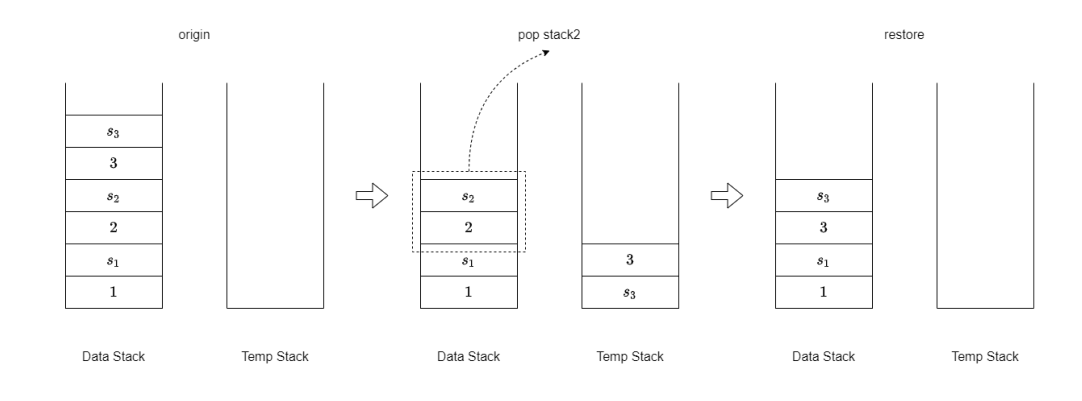
\includegraphics[width=1.0\textwidth,height=0.5\textwidth]{stack.png}
	\end{figure} \par
    So 3-PDAs are not more powerful than 2-PDAs.
\end{enumerate}
    
    \paragraph{Question 11 (with 1 bonus mark). Turing machine}~{}
    \\
    \begin{enumerate}
        \item [1.] Scan the input string from left to right to see whether the read symbol is a member of $\{0,1\}^*$. If there is a symbol which is not 0s or 1s,reject, otherwise go to step 2.
        \item [2.] Move the head to the left-hand end, and move to right until read a 0s, write 's' and go to step 3. If there is no 0s, go to step 4.
        \item [3.] Move the head to the left-hand end, and move to right until read a 1s, write 's' and go to step 2. If there is no 1s, reject.
        \item [4.] Move the head to the left-hand end, and scan from left to right, if there is a symbol other than 's', reject, otherwise accept.
    \end{enumerate}

    \paragraph{Question 12 (with 1 bonus mark). Decidability}~{}
    \\

    A is decidable. \par
    There are only 2 possibilities for set  A  : either  \{0\}  or  \{1\} , which are both finite sets and hence decidable.\par
    We can define a TM to decides it:
    Match the input string with the only string  $s$ in language. Accept if they match, and reject otherwise.\par
    Therefore, even though we don't know whether there will be reasonably-priced yummies in the canteens of NJU someday, the language  A  is decidable.
\end{document}
